\subsection{Software Development Process}
\label{subsec:soft_dev}
A modified Agile Software Development Methodology, was utilized in the development
of the alamSYS and its components, primarily due to the time constraints
on the conduct of this study. Wherein, Agile Sprints were primarily used to manage 
time efficiently during the software development process
\cite{JavaTPointAgile, Milne2021}. Moreover, shown in Figure \ref{fig:agile} was followed 
in the system development procedures for this special problem.

% Agile Development
\begin{figure}[ht]
    \centering
    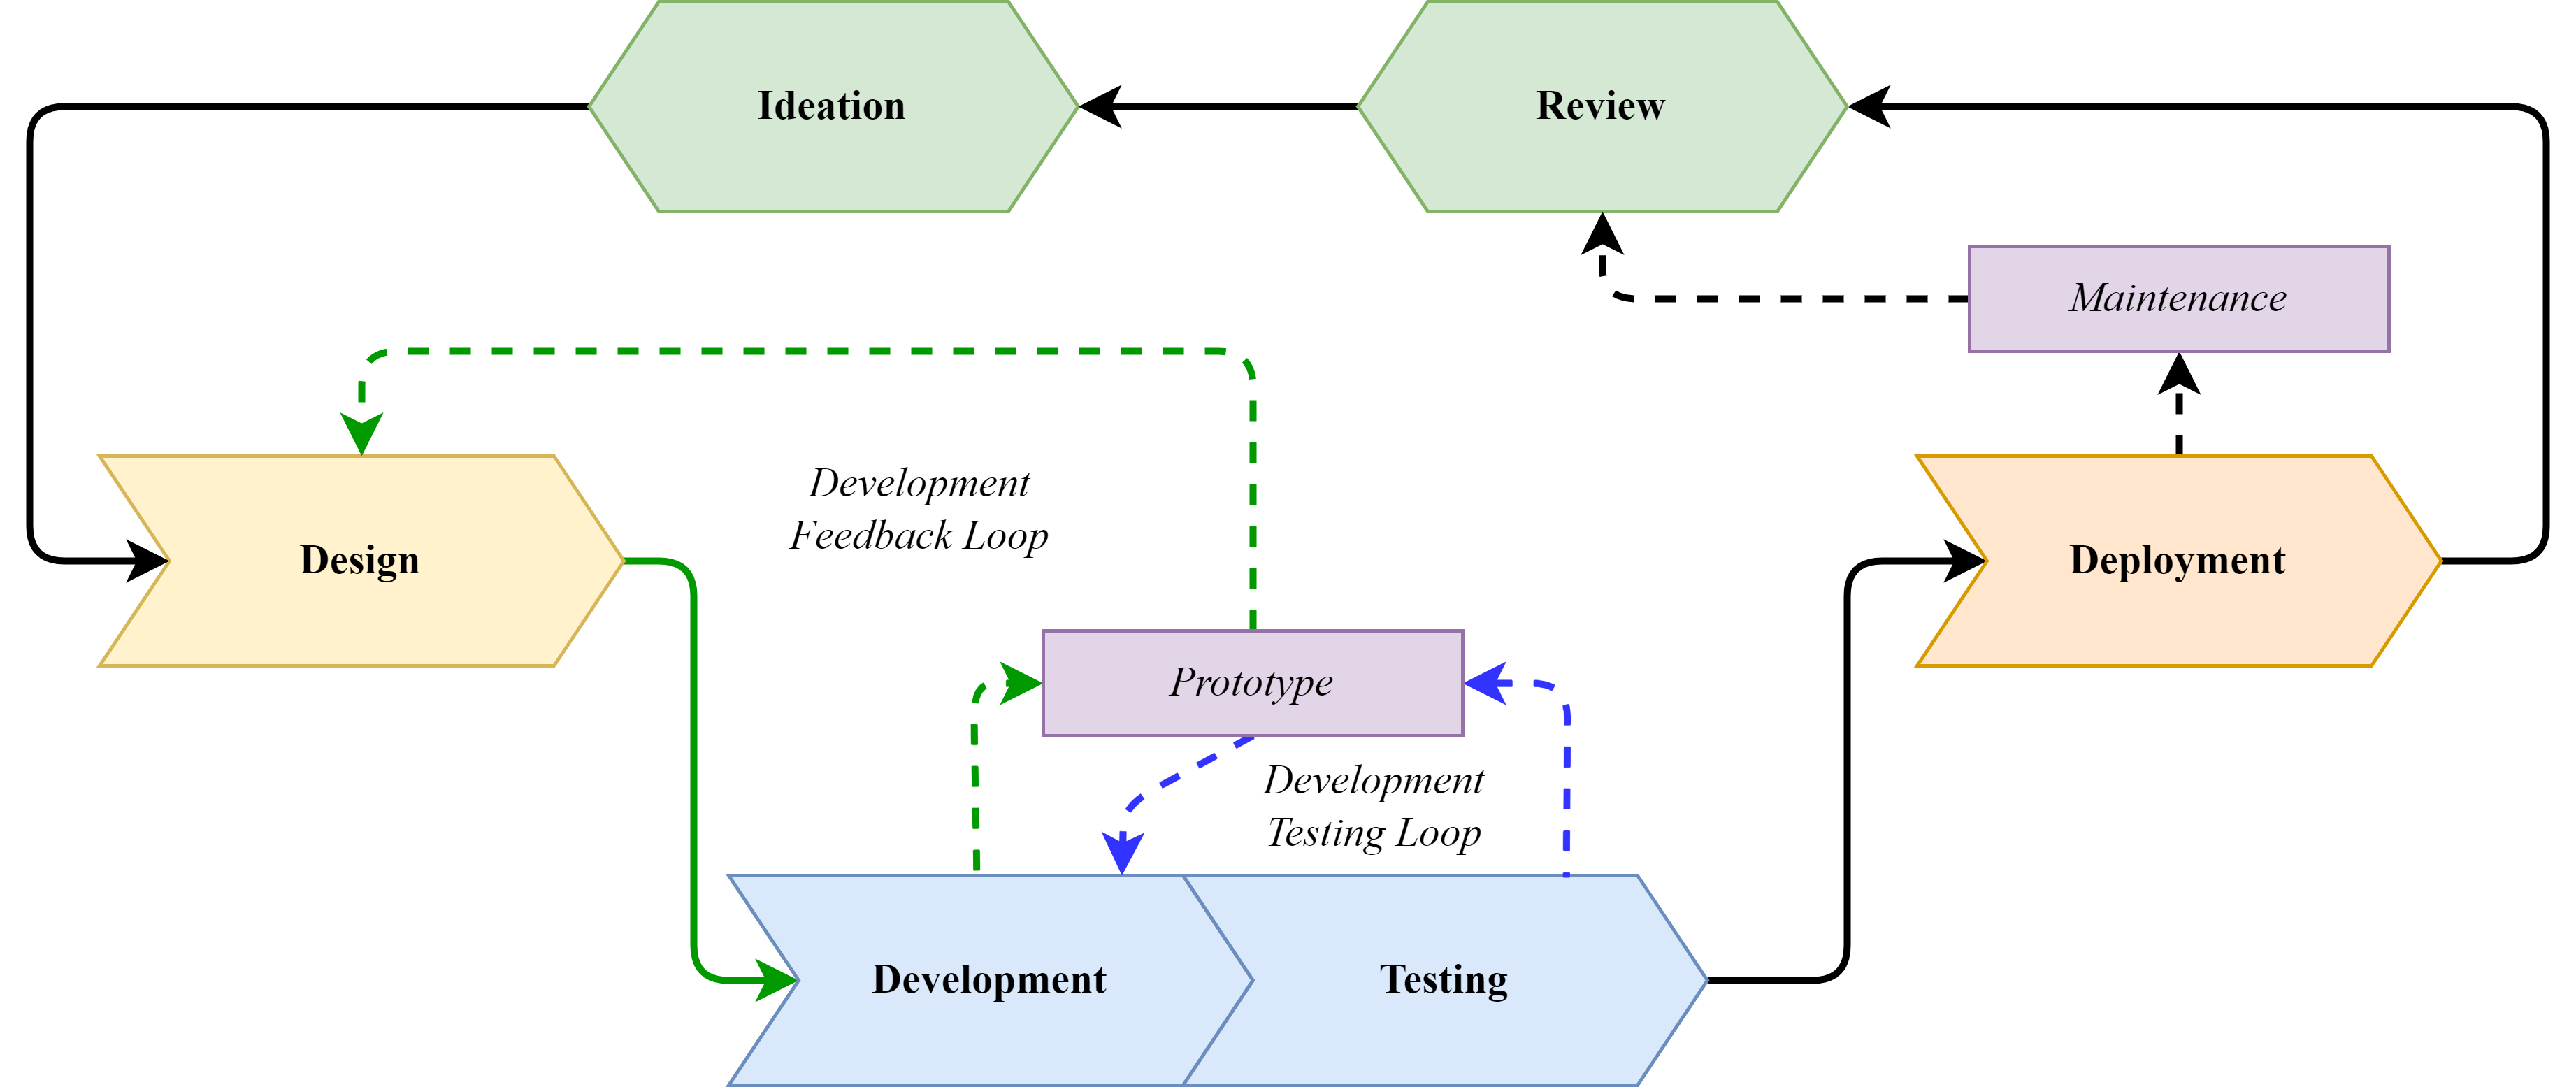
\includegraphics[width=1\textwidth]{./assets/Chapter_3/agile.png}
    \caption{Modified Agile Development Methodology}
    \label{fig:agile}
\end{figure}
\FloatBarrier

The modified agile development methodology shown above includes 
additional and specific "feedback loops" such as a development 
feedback loop that focuses on the continuous design and development 
process; and a development testing loop that ensures that the 
software being developed works as intended or better than expected.

\subsubsection{Summary of Agile Sprints}
\label{subsubsec:summ_sprints}
The following Agile Sprints are conducted in the development of the alamSYS and its components: 
(1) Requirement Analysis, System Planning, and Evaluation; (2) Development of Initial System Prototype; 
(3) Development and Testing of DMD-LSTM Model; (4) Integration of DMD-LSTM Model to the alamSYS, 
and Initial System Testing; (5) System Testing, Analysis, Refactoring, and Deployment; and 
(6) Finalization of Paper, System Defense, and Presentation. Table \ref{summary-sprints} in the Appendices section 
contains additional information on these sprints.